%\documentclass[iop]{emulateapj}
%\documentclass[12pt, preprint]{emulateapj}
\documentclass[12pt, onecolumn]{emulateapj}

\usepackage{amsmath}
%\usepackage{bibtex}
%\bibliographystyle{unsrtnat}

\usepackage{tikz}
\usetikzlibrary{shapes.geometric, arrows}
\usetikzlibrary{fit}

\tikzstyle{hyper} = [circle, text centered, draw=black]%, fill=blue!30]
\tikzstyle{param} = [circle, text centered, draw=black]%, fill=green!30]
\tikzstyle{data} = [circle, text centered, draw=black, line width=2pt]%, fill=red!30]
%\tikzstyle{hyper} = [trapezium, trapezium left angle=70, trapezium right angle=110, minimum width=1cm, minimum height=0.5cm, text centered, draw=black, fill=green!30]
%\tikzstyle{param} = [rectangle, minimum width=1cm, minimum height=0.5cm, text centered, draw=black, fill=green!30]
%\tikzstyle{data} = [diamond, minimum width=1cm, minimum height=1cm, text centered, draw=black, fill=red!30]
%\tikzstyle{eqn} = [rectangle, minimum width=1cm, minimum height=0.5cm, text centered, draw=black]%, fill=green!30]
%\tikzstyle{latent} = [diamond, minimum width=1cm, minimum height=0.5cm, text centered, draw=black]%, fill=green!30]
\tikzstyle{arrow} = [thick,->,>=stealth]

\newcommand{\myemail}{aimalz@nyu.edu}
\newcommand{\textul}{\underline}

%\slugcomment{}

\shorttitle{Probabilistic Redshifts}
\shortauthors{Malz}

\begin{document}

\begin{align}
\end{align}

\title{Photometric Redshift Estimation: Avenues for Improvement}

\author{A.I. Malz\altaffilmark{1}}
\altaffiltext{1}{CCPP}
\email{aimalz@nyu.edu}

\begin{abstract}
This document presents a brief introduction to photometric redshifts for a non-astronomer audience before outlining some open problems in the subject and a brief discussion of possible solutions.
\end{abstract}

\keywords{photo-z}

\section{Introduction}
\label{sec:intro}

Redshift is a measure of the relative velocity between an object and its observer.  It is of scientific relevance to obtain redshifts for galaxies in the universe, in part because the redshift $z$ is proportional to the distance $d$ by Hubble's Law.  Since light travels at a finite speed, more distant galaxies appear as they did at a distant time in the past, enabling study of galaxy evolution. 

The redshift may be observed by taking a spectrum, a measurement of the energy flux $f(\lambda)$ carried by photons from a galaxy over a range of wavelengths $\lambda$, and determining the displacement of recognizable features, such as atomic or molecular emission or absorption lines.  However, spectra are only available for the brightest galaxies, making them impractical for the study of distant galaxies.  The "poor man's" spectrum is photometry, an extremely coarse spectrum comprised of flux transmitted through each of several filters $q$ of transmittance $t_{q}(\lambda)$.

Given $Q$ filter throughputs $f_{q}$, an estimate of the initial spectrum $f(\lambda)$ is made.  This coarse spectrum is fit to a redshift either by assuming a library of physically motivated redshifted template spectra or by deriving an effective basis of spectral templates from a training set with spectroscopically confirmed redshifts.  Typically, the redshift we wish to estimate $\hat{z}$ is reported as the redshift $z^{t}$ of the best fit (as measured by $\chi^{2}$) template spectrum with some Gaussian error $\sigma^{2}$ based on the goodness of that fit and observational uncertainties on $f_{q}$.

Rather than making point estimates, it would be advantageous to estimate probability distribution functions (zPDFs) on redshifts of individual galaxies.  There are several interesting questions one may ask about such a procedure.  Before discussing these questions, let us establish some notation and review some background relevant to probability.

Let's say we have some data $\vec{d}_{n}$ from a galaxy $n$ in a survey of $N$ galaxies.  Though additional information may be included in $\vec{d}_{n}$, at the very least it must contain the $f_{q}^{n}$ that comprise the photometry.  Instead of being given energy fluxes $f_{q}^{n}$, we are sometimes provided with "magnitudes" $m_{q}^{n}\propto -\log f_{q}^{n}$.  In some cases, we are instead given $Q-1$ "colors" $c_{q}^{n}=m_{q+1}^{n}-m_{q}^{n}$ with one magnitude $m_{0}$ that may be used to calculate the original $\vec{m}_{n}$ from which the colors were derived.  We would like to use this data to estimate the parameter $z_{n}$ representing the galaxy's redshift.  

Point estimates $\hat{z}_{n}$ suffer from various weaknesses that affect the science we can do with them that are best illustrated by comparing $\hat{z}_{n}$ versus $z_{n}$ for a set of test data with known redshifts.  Since both template fitting and machine learning methods essentially match photometry to a template or basis spectrum with both an intrinsic spectrum and a redshift, there are errors associated with misassignment of both redshift and intrinsic spectra to $\vec{d}_{n}$.  "Catastrophic" errors occur when $|z_{n}-\hat{z}_{n}|$ is quite large, although another insidious type of error occurs when many galaxies near some $z$ sharing some feature are assigned redshift estimates near some $\hat{z}$ elsewhere. 

Instead, we would like to work with a redshift probability distribution function for each galaxy.  We recall Bayes' Theorem, the relationship between the likelihood $p(\vec{d}_{n}|z)$ (the probability of observing the data at each value of the continuous parameter $z$) and the posterior $p(z|\vec{d}_{n})$ (the probability of each value of the continuous parameter $z$ given the observed data): $p(\vec{d}_{n}|z)p(z)=p(z|\vec{d}_{n})p(\vec{d}_{n})$.  Because any estimate of redshift by template fitting or machine learning will implicitly have to be marginalized over some nuisance parameter $\alpha$ representing the estimator of the intrinsic spectrum, it is considered much easier to find the posterior $p(z|\vec{d}_{n})=\int p(z,\alpha|\vec{d}_{n})d\alpha$,which we shall refer to as zPDF from this point forward.

\section{Open Questions}

Here are some interesting questions we may ask about zPDFs:

\begin{enumerate}
%\item \label{it:likelihood} How can redshift likelihood functions, as opposed to posterior probability distributions, be estimated?
\item \label{it:posterior} What methods are appropriate and effective for generating posterior zPDFs from photometric data?
\item \label{it:single} How can one estimate a zPDF from a single band of photometry?
\item \label{it:plus} How much is an estimate of a zPDF improved by the inclusion of each additional band of photometry? 
\item \label{it:pixel} How can one use photometry at each pixel in a galaxy to generate a posterior zPDF?
\item \label{it:spatial} How informative is inclusion of the angular size of a galaxy to the estimated zPDF?
\item \label{it:position} How can the angular cross-correlation of galaxies be used to improve estimates of their zPDFs?
\end{enumerate}

These questions will each be discussed in detail below.

\subsection{Generation of zPDFs}

Question \ref{it:posterior} pertains to the processing of data $\vec{d}_{n}$ to estimate the distribution of parameters $p(z|\vec{d}_{n})$.  Prior work has employed similar methods to those used to obtain point estimates. Data-driven $k$-nearest neighbor algorithms have been implemented by \citet{she11} neglecting measurement errors and by \citet{bal08} including measurement errors.  \citet{car13} use prediction tree and random-forest classification techniques and \citet{car14} use self-organizing maps  to obtain zPDFs.  An extension of \citet{ben00} that produces full posteriors (as opposed to a selection of local maxima) from a template library has been discussed in the litertature, but a formal presentation has not yet been published.

\subsection{Single-band photometry}

Question \ref{it:single} is about the special case in which $\vec{d}_{n}=d_{n}$, a scalar.  If we were to calculate $p(z_{n}|d_{n})$ from such limited data, could it be used for meaningful inference?  I suspect $d_{n}$ would be a very noisy proxy for distance, since the flux is proportional to the inverse square of the distance to the source.  Noise would be introduced by the very characteristics in galaxy spectra that permit point estimates of redshift to be made.

\subsection{Marginals of multi-band photometry}

Question \ref{it:plus} is easy to answer given the answer to question \ref{it:single}.  In other words, how would the estimate of $p(z_{n}|\vec{d}_{n})$ change if the length of $\vec{d}_{n}$ were $Q+1$ instead of $Q$?  This could be done by repeating whatever procedure was done to answer question \ref{it:single} with the addition of another filter.

\subsection{Spatial information to refine zPDFs}

Question \ref{it:spatial} makes use of pixel-level data to incorporate discrepancies in photometry across the extent of a galaxy in the focal plane into the zPDF.

\subsection{Location information to refine zPDFs}

Question \ref{it:position} stems from the observed correlation of redshift between galaxies near one another on the sky, caused by the fact that many galaxies are interacting with their neighbors.  We shall use the sky coordinates $\vec{\phi}=(\alpha,\delta)$ in right ascension and declination.  For this discussion, let us say we have $N$ pairs of galaxies with data $\textul{d}_{n}$ comprised of photometry $\vec{f}_{n}$ and position $\vec{\phi}_{n}$ as well as $\textul{d}_{n'}$ comprised of photometry $\vec{f}_{n'}$, position $\vec{\phi}_{n'}$, and a reliable redshift $z_{n'}$.  

There are two current techniques in place for determining $z_{n}$.  The first is to set $\hat{z}_{n}=z_{n'}$ for all galaxies with $\theta_{n,n'}=\theta_{n',n}=|\vec{\phi}_{n'}-\vec{\phi}_{n}|$.  The second is to draw $\hat{z}_{n}$ from a normal distribution centered at $z_{n'}$ with a variance $\sigma^{2}_{n'}$ derived from some combination of $\theta$ and $z_{n'}$.  One possible approach to improving this method would be to work with $p(z_{n}|\textul{d}_{n})=N(z_{n'},\sigma^{2}_{n'})$.

A better solution takes advantage of our knowledge of the angular and/or redshift-space and/or real-space correlation functions $\vec{\xi}$ for galaxies.  Since these correlation functions are defined over all angular separations, we may relax the requirement that $\theta\ll1$.  By simultaneously inferring $z_{n}$ and $\vec{xi}$, we can improve both parameters.  Eq. \ref{eq:hyper} illustrates the approach.

\begin{align}
\label{eq:hyper}
p(z_{n},\vec{\xi}|\{\textul{d}_{n'}\}_{N})
\end{align}

Let us consider a survey in which $\vec{d}_{n}$ includes photometry and angular position $\vec{\theta}=(\alpha_{n},\delta_{n})$.  The physical distance between a pair of galaxies $n$ and $n'$ at $z_{k}$ is $R_{k}=d_{A}(z_{k})\cos^{-1}(\vec{\phi}_{n}\cdot\vec{\phi}_{n'})$.  An outline for answering this question may be intertpreted from the directed acyclic graph of Fig. \ref{fig:flow}.

\begin{figure}
\label{fig:flow}
\vspace{0.5cm}
\begin{center}
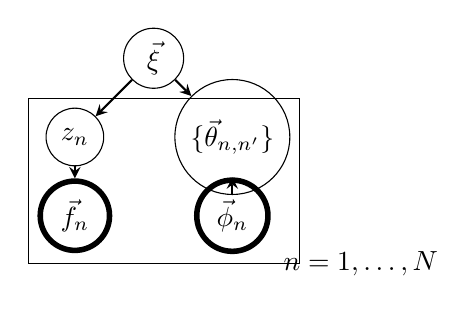
\begin{tikzpicture}[node distance=1cm]

\node (powspec) [hyper] {$\vec{\xi}$};
%\node (nz) [hyper, below of=powspec, xshift=-1cm] {$\vec{N}$};
%\node (croscor) [hyper, below of=powspec, xshift=+1cm] {$\vec{\xi}$};
\node (z) [param, below of=powspec, xshift=-1cm] {$z_{n}$};
\node (theta) [param, below of=powspec, xshift=+1cm] {$\{\vec{\theta}_{n,n'}\}$};
\node (mags) [data, below of=z] {$\vec{f}_{n}$};
\node (pos) [data, below of=theta] {$\vec{\phi}_{n}$};
\node (survey) [draw=black,fit={(mags.west)(z.north)(pos.south)(theta.east)}] {};
\node [xshift=2.5cm] at (survey.south) {$n=1,\dots,N$};

\draw [arrow] (powspec) -- (z);
\draw [arrow] (powspec) -- (theta);
%\draw [arrow] (nz) -- (z);
\draw [arrow] (z) -- (mags);
%\draw [arrow] (croscor) -- (theta);
\draw [arrow] (theta) -- (pos);

\end{tikzpicture}
\caption{This directed acyclic graph illustrates a hierarchical model in which the hyperparameters in the power spectrum determine the distributions of galaxy angular separations and redshifts, which are estimated from the data of observed magnitudes and positions.}
\end{center}
\end{figure}

\dots

\section{Applications}

zPDFs have been used in the literature to estimate parameters relevant to cosmology and galaxy evolution.  \citet{lop14} infers the merger fraction.  \citet{she11} infers the redshift density function $N(z)$.  \citet{mye09} infers the angular cross-correlation function $\vec{\xi}$.

%\acknowledgments

%\appendix

\bibliography{references}

\end{document}

First, let us establish some notation.  A galaxy $n$ in a survey of $N$ galaxies has an observed set of magnitudes in $Q$ bands that comprise a vector $\vec{m}_{n}$ of length $Q$.  Each filter has throughput over a spectrum of $S$ pixels that constitutes a vector $\vec{b}_{q}$ of length $S$.  These throughputs comprise the $Q\times S$ matrix $\textul{B}$.  There exists a spectral template library or training set of $K$ galaxies each with a spectrum $\vec{M}_{k}$ of length $S$.  The entire training set may be represented by a $S\times K$ matrix $\textul{T}$.  If the training set or template library spans the space of galaxies and each galaxy in the survey is uniquely drawn from that set, its observed photometry $\vec{m}_{j}$ may be represented by Eq. \ref{eq:zmod}, where $\hat{Z}_{j}$ represents the operator taking the template spectrum $\vec{t}_{k}$ from zero redshift to redshift $z_{j}$ of galaxy $j$ according to Eq. \ref{eq:kcorr}.

\begin{eqnarray}
\label{eq:zmod}
\vec{m}_{j} &=& \textul{B}\hat{Z}_{j}\vec{M}_{k} + \vec{e}_{j}
\end{eqnarray}

\begin{mathletters}
\begin{eqnarray}
\label{eq:kcorr}
\hat{Z}_{j}\vec{M}_{k} &=& 5(\log [(1+z_{j})\frac{c}{H_{0}}\int_{0}^{z_{j}}\frac{dz}{\sqrt{\Omega_{M}(1+z)^{3}+\Omega_{k}(1+z)^{2}+\Omega_{\Lambda}}}]-1)\\
&&+[M_{0,q}-2.5\log\frac{L_{q}}{L_{0,q}}]+[-2.5\log\left(\frac{1}{1+z_{j}}\frac{L'_{q'}}{L_{q}}\right)]\\
L_{q} &=& L_{q,0}10^{-\frac{(M_{q}-M_{q,0})}{2.5}}\nonumber
\end{eqnarray}
\end{mathletters}

In practice, a test set galaxy's photometry will have some probability of being a convolution of the filters and the spectrum of a training set galaxy at each possible redshift $z_{k}$.  To get the likelihood, one must set various values of the redshift and calculate the probability of the data given each of those values.  This corresponds to Eq. \ref{eq:pzk}.  I DON'T THINK THIS IS RIGHT!  

\begin{eqnarray}
\label{eq:pzk}
p(n|m,k) &\propto& \left((\textul{B}\hat{Z}_{k}\vec{t}_{m}-\vec{f}_{n})^{T}(\textul{B}\hat{Z}_{k}\vec{t}_{m}-\vec{f}_{n})\right)^{-1}
\end{eqnarray}

Then the probability distribution $p(n|k)$ will take the form of \ref{eq:pz}.  For the training set galaxies, $p(m|k)$ is simply 1 for $z_{m}=z_{k}$ and 0 otherwise and $p(n|m,k)$ is given by Eq. \ref{eq:pzk}.

\begin{eqnarray}
\label{eq:pz}
p(n|k) &\propto& \sum_{m=1}^{M}p(n|m,j)p(m|k)
\end{eqnarray}

Because the LSST simulations publish the input catalog for the images, the redshifts of all galaxies and their true spectra are known in addition to the flux in several bands at every pixel, hence question \ref{it:pixel}.  If $p(n|k,(i,j))$ were known at every pixel $(i,j)$, how would one calculate $p(n|k)$ for the entire galaxy?  I could use some kind of weighting scheme based on how representative $\vec{f}_{n}(i,j)$ is of the integrated flux $\vec{f}_{n}$.